\chapter{\normalfont SUPPLEMENTARY MATERIAL FOR CHAPTER 2}
\label{ch:cha2_supp}
\newpage

\section*{\normalfont True Parameters for 100 Simulations }
\footnotesize
\begin{xltabular}{\textwidth}{X X X X X X X X}
\toprule
$\sigma_{AC}$ & $\sigma_{AG}$ &  $\sigma_{AT}$ &  $\sigma_{CG}$ &  $\sigma_{CT}$ &  $\sigma_{GT}$ & $\omega$ &  $\tau$
\endfirsthead
$\sigma_{AC}$ & $\sigma_{AG}$ &  $\sigma_{AT}$ &  $\sigma_{CG}$ &  $\sigma_{CT}$ &  $\sigma_{GT}$ & $\omega$ &  $\tau$
\\\hline
\endhead 
\midrule  
\csvreader[]{cha1/table/true_par_tab.csv}{}  
{\\ \csvcoli&\csvcolii&\csvcoliii &\csvcoliv &\csvcolv &\csvcolvi &\csvcolvii &\csvcolviii}  
\\ \bottomrule
\caption{True Parameters for 100 Simulations.}
\end{xltabular}
\label{tab:true_par}

\section*{\normalfont Parameter Estimates of 100 Simulations in The Codon Length of $10^5$ via Phylo-Em Method}
\footnotesize
\begin{xltabular}{\textwidth}{X X X X X X X X}
\toprule
$\sigma_{AC}$ & $\sigma_{AG}$ &  $\sigma_{AT}$ &  $\sigma_{CG}$ &  $\sigma_{CT}$ &  $\sigma_{GT}$ & $\omega$ &  $\tau$
\endfirsthead
$\sigma_{AC}$ & $\sigma_{AG}$ &  $\sigma_{AT}$ &  $\sigma_{CG}$ &  $\sigma_{CT}$ &  $\sigma_{GT}$ & $\omega$ &  $\tau$
\\\hline
\endhead
\midrule
\csvreader[]{cha1/table/est_5e_tab.csv}{}
{\\ \csvcoli&\csvcolii&\csvcoliii &\csvcoliv &\csvcolv &\csvcolvi &\csvcolvii &\csvcolviii}
\\ \bottomrule
\caption{Parameter Estimates of 100 Simulations in The Codon Length of $10^5$ via Phylo-Em Method.}
\end{xltabular}
\label{tab:em_par}

\section*{\normalfont Parameter Estimates of 100 Simulations in The Codon Length of $10^5$ via Nmkb Method}
\footnotesize
\begin{xltabular}{\textwidth}{X X X X X X X X}
\toprule
$\sigma_{AC}$ & $\sigma_{AG}$ &  $\sigma_{AT}$ &  $\sigma_{CG}$ &  $\sigma_{CT}$ &  $\sigma_{GT}$ & $\omega$ &  $\tau$
\endfirsthead
$\sigma_{AC}$ & $\sigma_{AG}$ &  $\sigma_{AT}$ &  $\sigma_{CG}$ &  $\sigma_{CT}$ &  $\sigma_{GT}$ & $\omega$ &  $\tau$
\\\hline
\endhead
\midrule
\csvreader[]{cha1/table/est_5e_tab.csv}{}
{\\ \csvcoli&\csvcolii&\csvcoliii &\csvcoliv &\csvcolv &\csvcolvi &\csvcolvii &\csvcolviii}
\\\bottomrule
\caption{Parameter Estimates of 100 Simulations in The Codon Length of $10^5$ via Nmkb Method.}
\end{xltabular}
\label{tab:nmkb_par}

\section*{\normalfont Parameter Estimates of 90 Species Pairs}
\footnotesize
\begin{xltabular}{\textwidth}{X X| X X X X X X X X}
\toprule
Species & & $\sigma_{AC}$ & $\sigma_{AG}$ &  $\sigma_{AT}$ &  $\sigma_{CG}$ &  $\sigma_{CT}$ &  $\sigma_{GT}$ & $\omega$ &  $\tau$
\endfirsthead
Species & & $\sigma_{AC}$ & $\sigma_{AG}$ &  $\sigma_{AT}$ &  $\sigma_{CG}$ &  $\sigma_{CT}$ &  $\sigma_{GT}$ & $\omega$ &  $\tau$
\\\hline
\endhead
\midrule
\csvreader[]{cha1/table/est_90_tab.csv}{}
{\\ \csvcoli & & \csvcolii&\csvcoliii &\csvcoliv &\csvcolv &\csvcolvi &\csvcolvii &\csvcolviii &\csvcolix}
\\ \bottomrule
\caption{Parameter Estimates of 90 Species Pairs.}
\end{xltabular}
\label{tab:90_par}

%%%%%%%%%%%%%%%%%%%%%%%%%%%%%%%%%%%%%%%%%%%%%%%%%%%%%%%%%%%%%
\chapter{\normalfont SUPPLEMENTARY MATERIAL FOR CHAPTER 3}
\label{ch:cha3_supp}
\newpage

\section*{\normalfont File Size Change in the Pipeline}
\footnotesize
\begin{table}[H]
\centering
\begin{tabularx}{\textwidth}{X X}
\toprule
Pipeline step & File size \\
\midrule
Homologous genes & 14547 \\
Sequence alignments & 13827 \\
Gaps curation & 2034, 1712, 1652, 1605 \\
\bottomrule
\end{tabularx}
\titlecaption{File Size Change in the Pipeline.}{The bottom step has four different file sizes because we use four window sizes.}
\label{tab:file_size}
\end{table}

\section*{\normalfont Phase Proportions of Insertion and Deletion Events across Four Window Sizes}
\footnotesize
\begin{xltabular}{\textwidth}{X X|X X X|X X X|X X X|X X X}
\toprule
& & \multicolumn{3}{c|}{\textbf{window size of 3}} & \multicolumn{3}{c|}{\textbf{window size of 6}} & \multicolumn{3}{c}{\textbf{window size of 9}}& \multicolumn{3}{c}{\textbf{window size of 12}}\\
\midrule  
 & & P0 & P1 & P2 & P0 & P1 & P2 & P0 & P1 & P2 & P0 & P1 & P2 \\
\bottomrule
\csvreader[]{cha2/table/Phase.prop.test.csv}{}  
{\\ \csvcoli & &\csvcolii&\csvcoliii &\csvcoliv &\csvcolv &\csvcolvi &\csvcolvii &\csvcolviii &\csvcolix &\csvcolx &\csvcolxi &\csvcolxii &\csvcolxiii}  
\\ \hline
\titlecaption{Phase Proportions of Insertion and Deletion Events across Four Window Sizes.}{Insertion and Deletion rows represent the proportion of indel phases in each window size. The P.value row represent the p value of testing the null that the proportion of a specific phase is equal between insertion and deletion groups.} 
\end{xltabular}
\label{tab:pha_ins_del}



%%%%%%%%%%%%%%%%%%%%%%%%%%%%%%%%%%%%%%%%%%%%%%%%%%%%%%%%%%%%%%%%%%%%
\chapter{\normalfont SUPPLEMENTARY MATERIAL FOR CHAPTER 4}
\label{ch:cha4_supp}
\newpage

\section*{\normalfont True Parameters for 100 Simulations}
\footnotesize
\begin{xltabular}{\textwidth}{X X X X X X X X X X X X X}
\toprule
$\sigma_{AC}$ & $\sigma_{AG}$ & $\sigma_{AT}$ & $\sigma_{CG}$ & $\sigma_{CT}$ & $\sigma_{GT}$ & $\omega$ & $\tau$ & ext.I & ext.D & r0 & r1 & r2 
\endfirsthead
$\sigma_{AC}$ & $\sigma_{AG}$ & $\sigma_{AT}$ & $\sigma_{CG}$ & $\sigma_{CT}$ & $\sigma_{GT}$ & $\omega$ & $\tau$ & ext.I & ext.D & r0 & r1 & r2 
\\\hline
\endhead
\midrule
\csvreader[]{cha3/table/true_par.csv}{}
{\\ \csvcoli &\csvcolii &\csvcoliii &\csvcoliv &\csvcolv &\csvcolvi &\csvcolvii &\csvcolviii
&\csvcolix &\csvcolx &\csvcolxi &\csvcolxii &\csvcolxiii}
\\ \bottomrule
\titlecaption{True Parameters for 100 Simulations.}{ext.I and ext.D are gap extension weight of insertions and deletions, with codon length as the unit; r0, r1, r2 are the indel phase rates over the branch length.}
\end{xltabular}
\label{tab:true_par_cha3}

\section*{\normalfont 100 Parameter Estimates via Gillespie Simulation Method}
\footnotesize
\begin{xltabular}{\textwidth}{X X X X X X X X X X X X X}
\toprule
$\sigma_{AC}$ & $\sigma_{AG}$ & $\sigma_{AT}$ & $\sigma_{CG}$ & $\sigma_{CT}$ & $\sigma_{GT}$ & $\omega$ & $\tau$ & ext.I & ext.D & r0 & r1 & r2 
\endfirsthead
$\sigma_{AC}$ & $\sigma_{AG}$ & $\sigma_{AT}$ & $\sigma_{CG}$ & $\sigma_{CT}$ & $\sigma_{GT}$ & $\omega$ & $\tau$ & ext.I & ext.D & r0 & r1 & r2 
\\\hline
\endhead
\midrule
\csvreader[]{cha3/table/sim_par.csv}{}
{\\ \csvcoli &\csvcolii &\csvcoliii &\csvcoliv &\csvcolv &\csvcolvi &\csvcolvii &\csvcolviii
&\csvcolix &\csvcolx &\csvcolxi &\csvcolxii &\csvcolxiii}
\\ \bottomrule
\caption{100 Parameter Estimates via Gillespie Simulation Method.}
\end{xltabular}
\label{tab:sim_par_cha3}

\section*{\normalfont 100 Parameter Estimates via Importance Sampling Method within EM}
\footnotesize
\begin{xltabular}{\textwidth}{X X X X X X X X X X X X X}
\toprule
$\sigma_{AC}$ & $\sigma_{AG}$ & $\sigma_{AT}$ & $\sigma_{CG}$ & $\sigma_{CT}$ & $\sigma_{GT}$ & $\omega$ & $\tau$ & ext.I & ext.D & r0 & r1 & r2 
\endfirsthead
$\sigma_{AC}$ & $\sigma_{AG}$ & $\sigma_{AT}$ & $\sigma_{CG}$ & $\sigma_{CT}$ & $\sigma_{GT}$ & $\omega$ & $\tau$ & ext.I & ext.D & r0 & r1 & r2 
\\\hline
\endhead
\midrule
\csvreader[]{cha3/table/im_par.csv}{}
{\\ \csvcoli &\csvcolii &\csvcoliii &\csvcoliv &\csvcolv &\csvcolvi &\csvcolvii &\csvcolviii
&\csvcolix &\csvcolx &\csvcolxi &\csvcolxii &\csvcolxiii}
\\ \bottomrule
\caption{100 Parameter Estimates via Importance Sampling Method within EM.}
\end{xltabular}
\label{tab:im_par_cha3}


%%%%%%%%%%%%%%%%%%%%%%%%%%%%%%%%%%%%%%%%%%%%%%%%%%%%%%%%%%%%%
\chapter{\normalfont SUPPLEMENTARY MATERIAL FOR CHAPTER 5}
\label{ch:cha4_supp}
\newpage

\section*{\normalfont Pairwise Species Number 1-16 Name Extension Table}
\footnotesize
{\RaggedRight 
\begin{table}[ht]
\renewcommand{\arraystretch}{1}
\begin{tabular}{p{0.2\linewidth} p{0.4\linewidth} p{0.3\linewidth}}
\hline
Species & Taxon name & Common name \\\\
\hline
01FcaCaf        & Canis lupus familiaris, Felis catus               & Dog, Cat\\
02MusRat        & Mus musculus, Rattus norvegicus                   & Mouse, Rat\\
03HsaMmu        & Homo sapiens, Macaca mulatta                      & Human, Macaca\\
04Gallus        & Gallus gallus, Meleagris gallopavo                & Chicken, Wild turkey\\
05Droso         & Drosophila sechellia, Drosophila simulans         & Fruit fly\\
06Nematode      & NA                                                & Roundworm genus\\
07yeast         & Saccharomyces cerevisiae, Saccharomyces paradoxus & Yeast, Wild yeast\\
08Arab          & Arabidopsis thaliana, Arabidopsis lyrata          & Thale cress,Sand Cress\\
09SarMon        & Monodelphis domestica, Sarcophilus harrisii       & Short-tailed opossum, Tasmanian devil\\
10ants          & Atta cephalotes, Solenopsis invicta               & Leaf cutting ant, Red imported fire ant\\
11malaria       & Plasmodium vivax, Plasmodium knowlesi             & Malaria parasite genus\\
12fugu          & Takifugu rubripes, Tetraodon nigroviridis         & Japanese puffer, Spotted green pufferfish \\
13Phytophthora  & Phytophthora infestans, Phytophthora parasitica   & Potato blight, Black shank\\
14Fusarium      & Fusarium graminearum, Fusarium pseudograminearum  & Gibberella zeae, Crown rot\\
15Oryza         & Oryza sativa Japonica, Oryza glaberrima           & Asian rice, African rice\\
16Solanum       & Solanum tuberosum, Solanum lycopersicum           & Potato, Tomato\\
\hline
\end{tabular}
\caption{Pairwise Species Number 1-16 Name Extension Table}
\end{table}}
\label{tab:spec_name}
\newpage

\section*{\normalfont Phase Proportions of 90 Species across Three Alignment Methods}
\footnotesize
\begin{xltabular}{\textwidth}{X X X| X X X| X X X| X X X}
\toprule
& & & \multicolumn{3}{c|}{\textbf{mafft+sw}} & \multicolumn{3}{c|}{\textbf{coati-max}} & \multicolumn{3}{c}{\textbf{coati-sampling}}\\
\midrule  
Species & & & P0 & P1 & P2 & P0 & P1 & P2 & P0 & P1 & P2 \\
\endfirsthead
Species & & & P0 & P1 & P2 & P0 & P1 & P2 & P0 & P1 & P2 \\
\hline
\endhead 
\bottomrule
\csvreader[]{cha4/table/phase_prop_all.csv}{}  
{\\ \csvcoli & & &\csvcolii&\csvcoliii &\csvcoliv &\csvcolv &\csvcolvi &\csvcolvii &\csvcolviii
&\csvcolix &\csvcolx}  
\\ \hline
\titlecaption{Phase Proportions of 90 Species across Three Alignment Methods}{P0--Phase0, P1--Phase1, P2-Phase2.} 
\end{xltabular}
\label{tab:phase_prop_all}

\section*{\normalfont dN/dS and Zn/(Zn+Zs) Ratio of 90 Species across Three Alignment Methods}
\footnotesize
\begin{xltabular}{\textwidth}{X X| X X| X X| X X}
\toprule
& & \multicolumn{2}{c|}{\textbf{mafft+sw}} & \multicolumn{2}{c|}{\textbf{coati-max}} & \multicolumn{2}{c}{\textbf{coati-sampling}}\\
\midrule  
Species & & dN/dS & Zn/Zn+Zs & dN/dS & Zn/Zn+Zs & dN/dS & Zn/Zn+Zs \\
\endfirsthead
Species & & dN/dS & Zn/Zn+Zs & dN/dS & Zn/Zn+Zs & dN/dS & Zn/Zn+Zs \\
\hline
\endhead 
\bottomrule
\csvreader[]{cha4/table/dnds_ZnZs.csv}{}  
{\\ \csvcoli & &\csvcolii&\csvcoliii &\csvcoliv &\csvcolv &\csvcolvi &\csvcolvii}  
\\ \hline
\caption{dN/dS and Zn/(Zn+Zs) Ratio of 90 Species across Three Alignment Methods.} 
\end{xltabular}
\label{tab:dnds_ZnZs}

\section*{\normalfont ML Estimates of omega and Normalized Indel Rates r}
\footnotesize
\begin{xltabular}{\textwidth}{X X| X X X X}
\toprule
Species & & \bfseries $\omega$ & r0.norm & r1.norm & r2.norm \\
\endfirsthead
Species & & \bfseries $\omega$ & r0.norm & r1.norm & r2.norm \\
\hline
\endhead 
 \bottomrule 
\csvreader[]{cha4/table/omega_r.csv}{}  
{\\ \csvcoli & &\csvcolii&\csvcoliii &\csvcoliv &\csvcolv}  
\\ \hline
\titlecaption{MLE Estimates of $\omega$ and Normalized Indel Rates r.}{r0.norm, r1.norm, and r2.norm are normalized rates of phase0, phase1, and phase2 indel events.} 
\end{xltabular}
\label{tab:omega_r}
\newpage


%%%%%%%%%%%%%%%%%%%%%%%%%%
\section*{\normalfont Post-filtering Distance Distribution Plot of 90 Species}
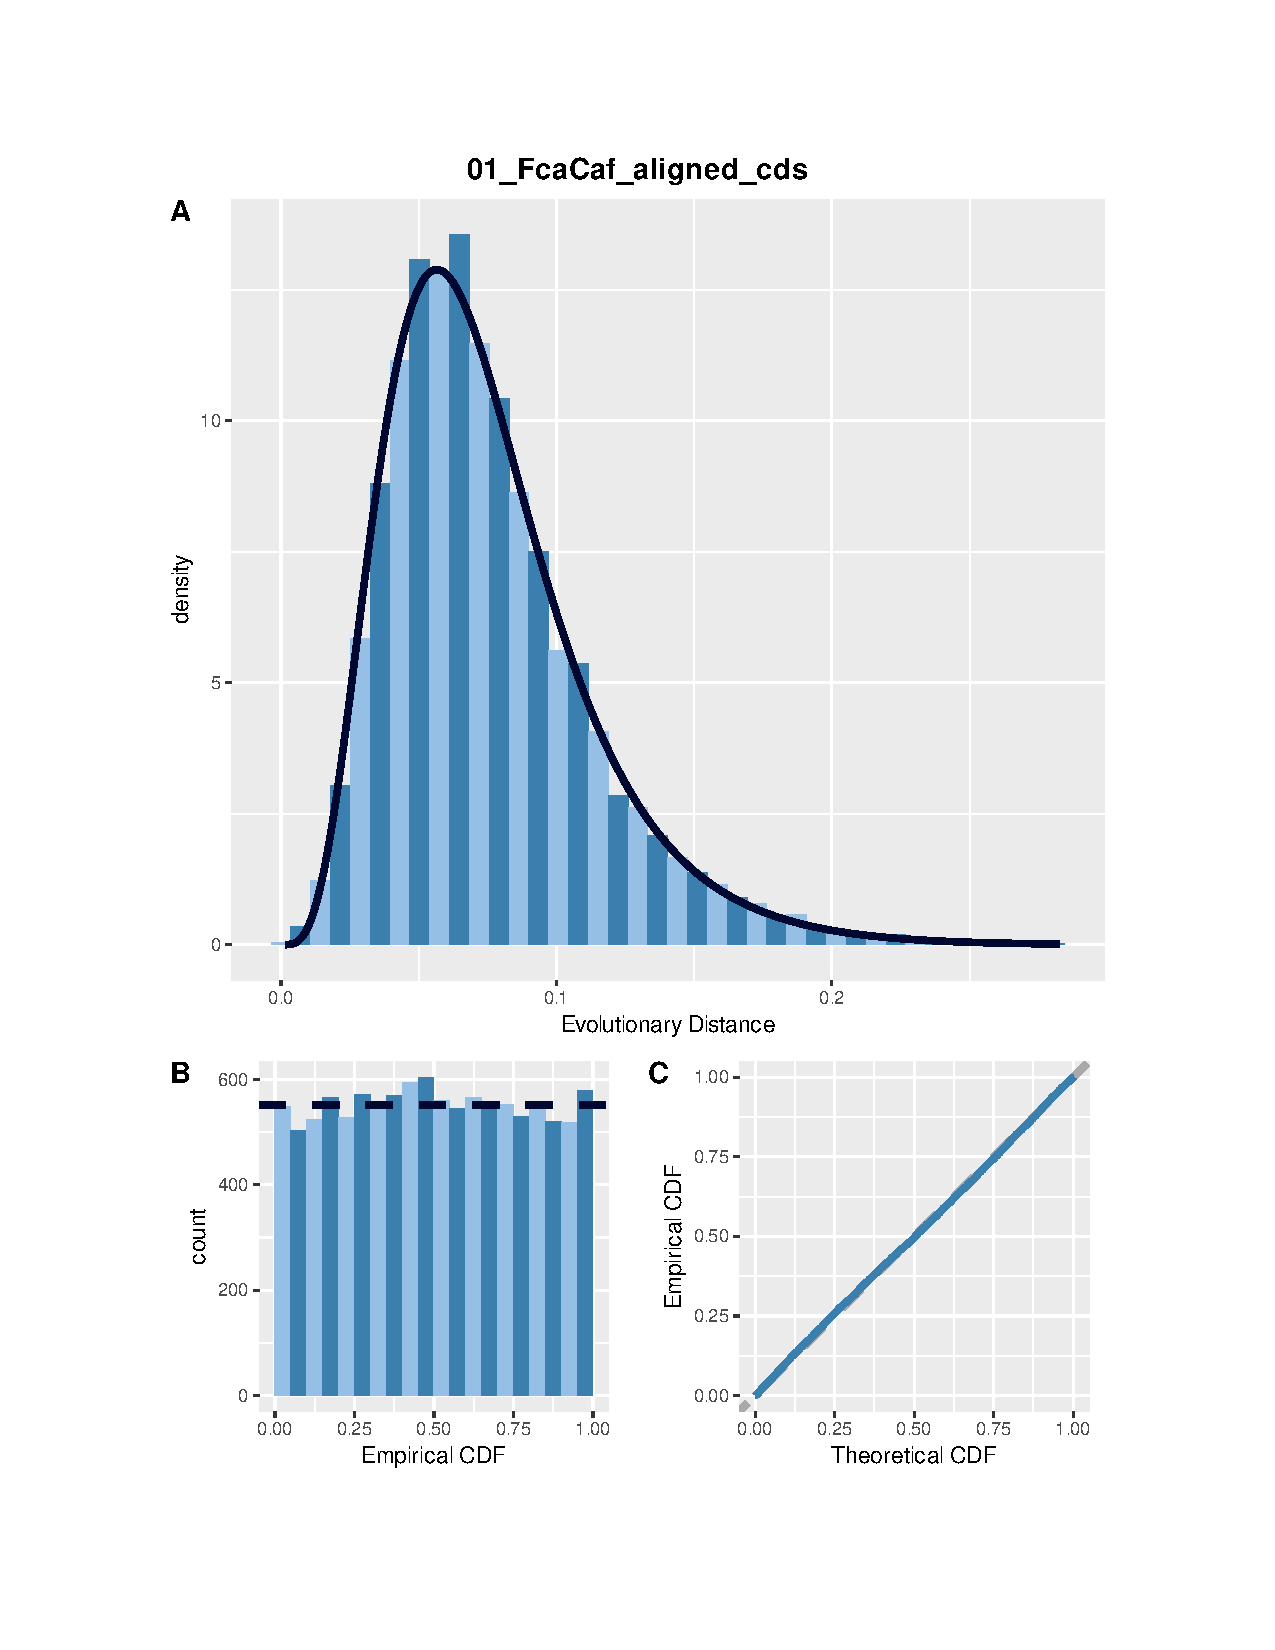
\includepdf[pages=-,scale=.8,pagecommand={}]{cha4/Figure/qc.pdf}
\begin{figure}[H]
     \centering
     \titlecaption{Post-filtering Distance Distribution Plot of 90 Species}
      {\footnotesize {A-plot is the evolutionary distance per gene pair that approximates a mixture gamma distribution (components=2). B-plot is the empirical CDF of the distance that follows an uniform distribution roughly, and C-plot is a Q-Q plot between the theoretical CDF and the empirical CDF of the distance data.}
      \par}
\end{figure}
\label{fig:post_fil}

\section*{\normalfont Histogram and QQplot of Phase Proportions of 90 Species}
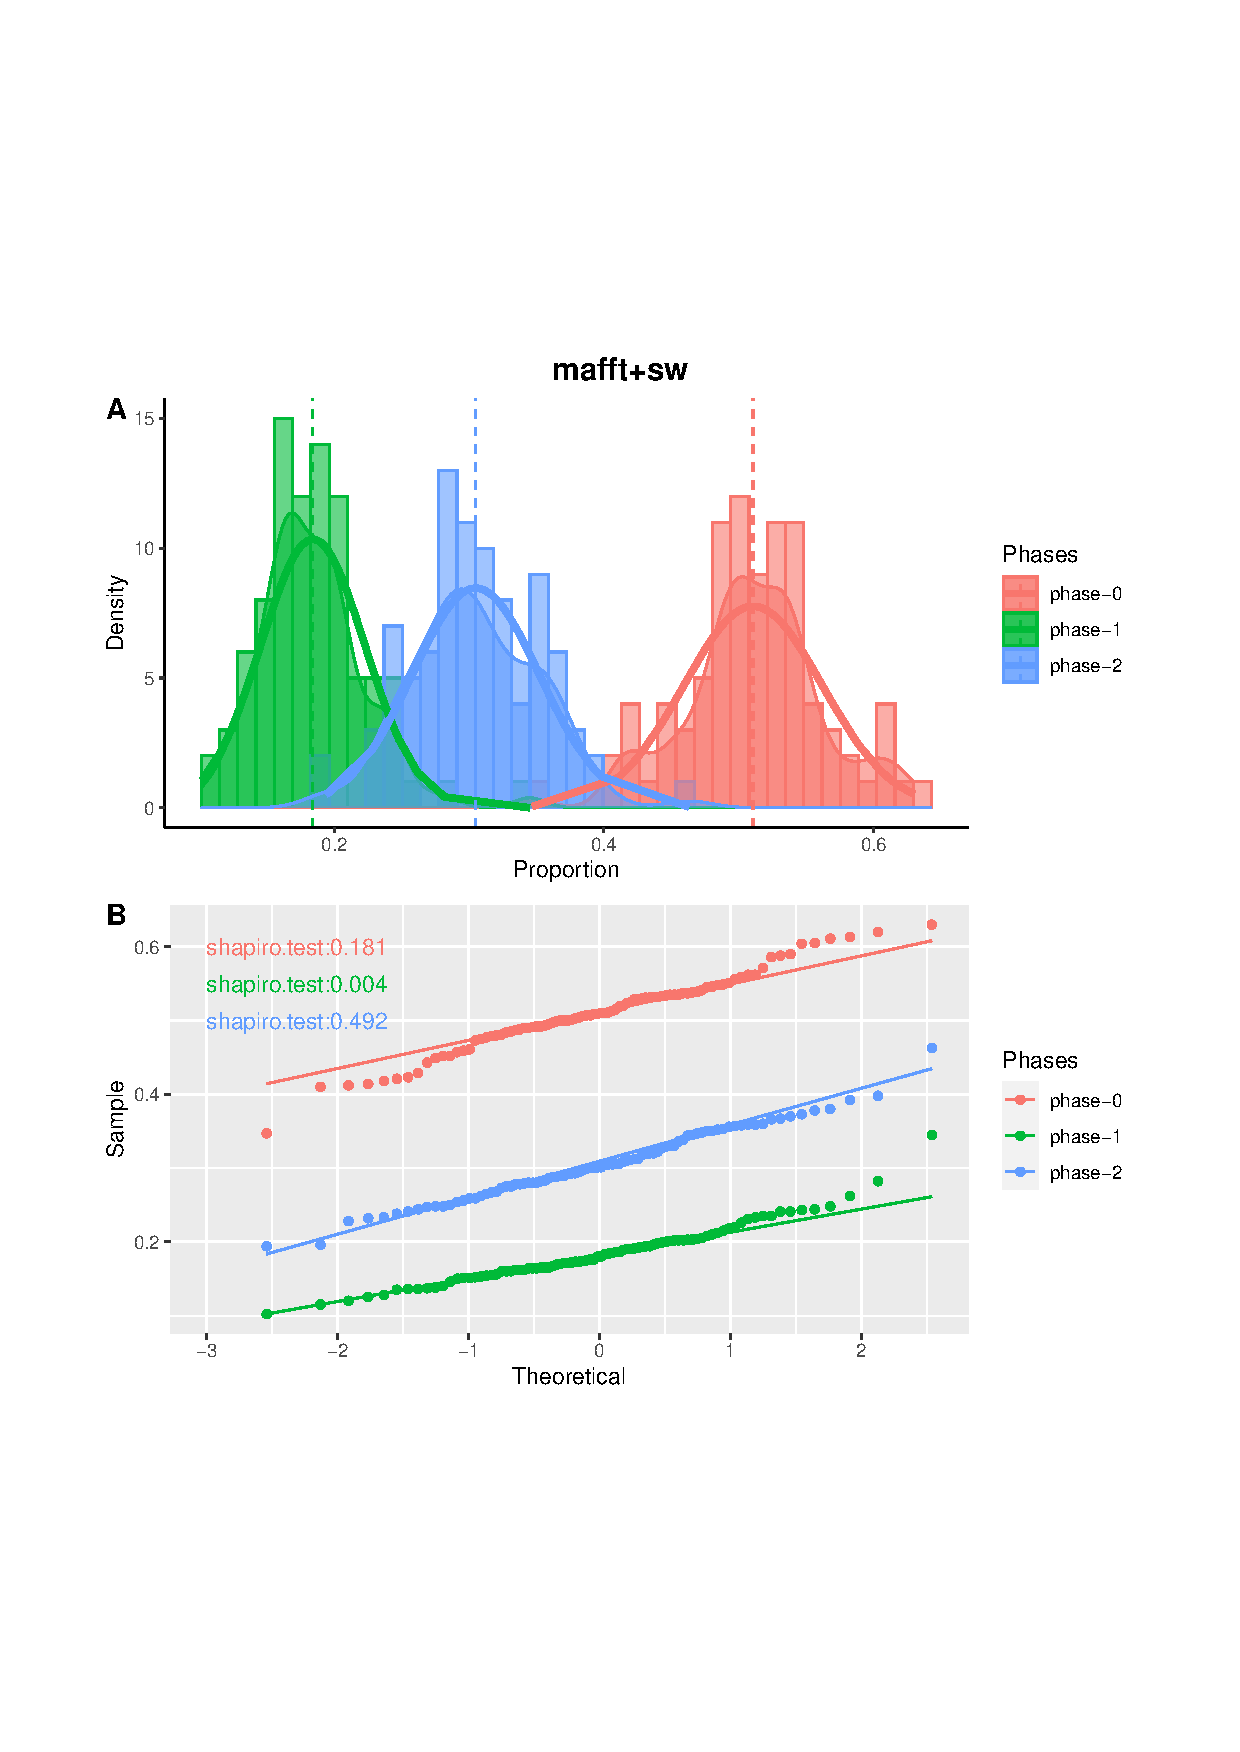
\includepdf[pages=-,scale=.8,pagecommand={}]{cha4/Figure/phase_prop.pdf}
\begin{figure}[H]
     \centering
     \titlecaption{Histogram and QQplot of Phase Proportions of 90 Species}
      {\footnotesize {Upper figure: The dashed line indicates the mean of each distribution, the thick curve is the shape of normal distribution. Lower figure: QQplot, the solid line is the straight diagonal line of each sample distribution.}
      \par}
\end{figure}
\label{fig:pha_prop}

\newpage
\section*{\normalfont Correlation Plot between Dnds and Zn/(Zn+Zs) of 90 Species}
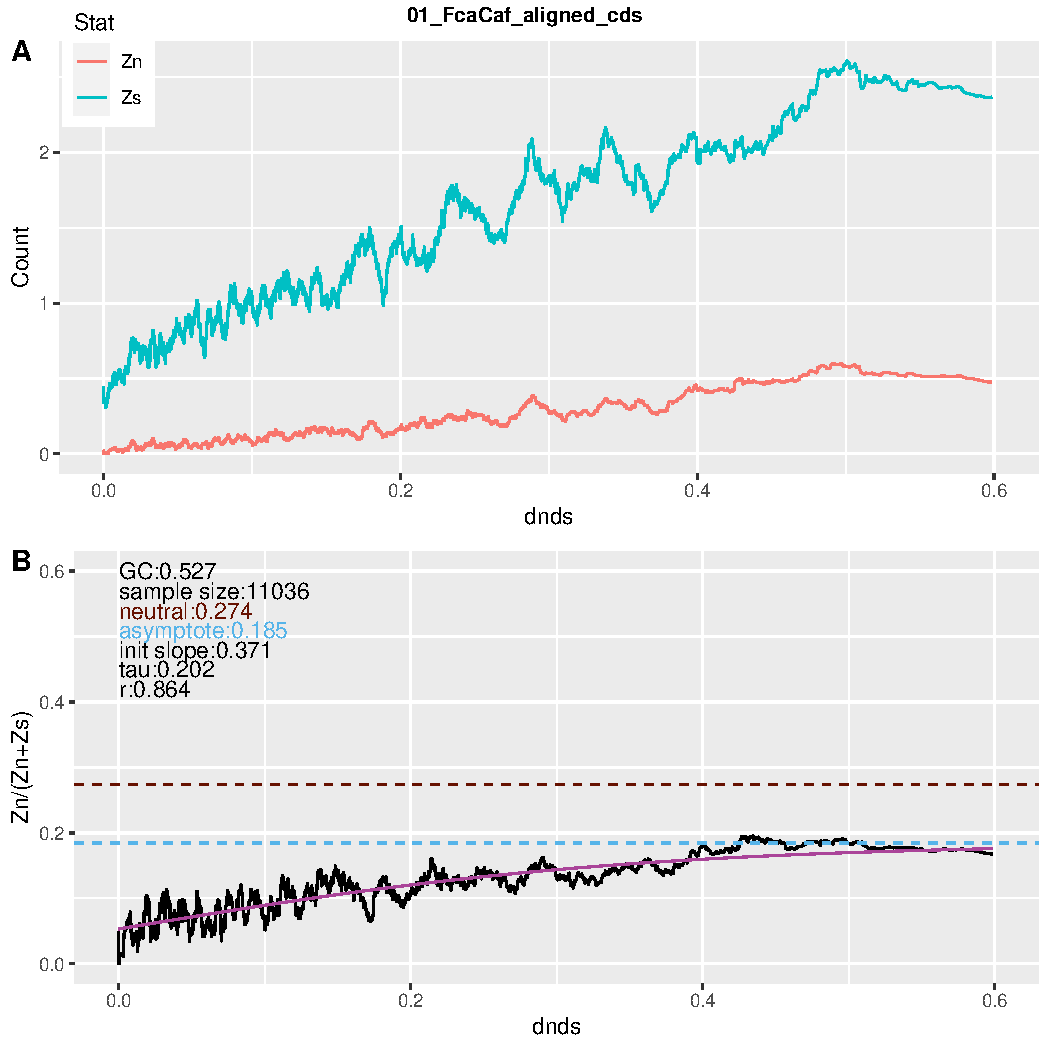
\includepdf[pages=-,scale=0.65,pagecommand={}]{cha4/Figure/roll_ZnZs_max.pdf}
\begin{figure}[H]
     \centering
     \caption{Correlation Plot between Dnds and Zn/(Zn+Zs) of 90 Species}
\end{figure}
\label{fig:dnds_ZnZs_corr}











